\documentclass{article}

\usepackage[T1]{fontenc}
\usepackage[spanish]{babel} %paquete para poner cosas en español
\usepackage{titling} %paquete para modificar el espaciado de los titulos
\usepackage[margin=.8in]{geometry} %paquete para poner márgenes más pequeños
\usepackage{titlesec} %paquete para modificar como se ven los titulos
\usepackage{graphicx} %paquete para meter imagenes
\usepackage{todonotes} %paquete para hacer \todo
\usepackage{hyperref}
\hypersetup{ %Setup of hyperref package
	 colorlinks=true,
	 linkcolor=black,
	 filecolor=brown,		
	 urlcolor=blue,
	 pdftitle={TP3 Digitales},
	 }
\usepackage{minted}
\usepackage{float}

\graphicspath{{imagenes/}}

\titleformat{\section}
	{\bfseries \huge}
	{}
	{0em}
	{}[\titlerule]

\titleformat{\subsection}
	{\bfseries \Large}
	{}
	{0em}
	{}

\titleformat{\subsubsection}
	{\bfseries \large}
	{}
	{0em}
	{}

\titlespacing{\section} %me permite controlar el espaciado de la seccion que le indico
	{0em}
	{3em}
	{1.5em}

\newcommand{\sectionbreak}{\clearpage}
\renewcommand{\labelenumi}{\alph{enumi})}
%
%
%

\begin{document}
\begin{titlepage}
	 \begin{center}
		 \vspace*{1cm}
				
		 {\Huge
		 \textbf{Trabajo Práctico Número 3}}
				
		 \vspace{0.3cm}
		 {\LARGE
		 Informe técnico	}
		 
		\vspace{0.5cm}
		 {\Large
		Un trabajo presentado para la materia de \\
		 Aplicaciones de electrónica digital}
				
		\vspace{1.5cm}
		 \begin{figure}[H]
		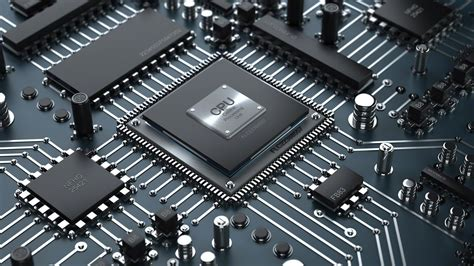
\includegraphics[width=0.6\textwidth]{logo}
		\centering
		\end{figure}
		\vfill
		 {\Large
		 \textbf{Krapp Ramiro -- Golmar Elias -- Pisacane Juan Cruz} \\
		 Instituto tecnológico San Bonifacio\\
		 Departamento de electrónica\\}
		 \today
		 
		 \vspace{0.5cm}
		 {\large Hecho en \LaTeX}

	 \end{center}
\end{titlepage}

\setcounter{tocdepth}{3}
\tableofcontents
\noindent\rule{\textwidth}{0.7pt}

\section{Actividad}
Se desea realizar una cerradura electrónica.

La misma debe contener como entrada un control de acceso por teclado (matricial);
como salidas dos señales de 12V para el accionamiento de un solenoide
(consumo máximo 150mA) y un zumbador (consumo máximo 50mA).

El circuito debe permitir 3 (tres) intentos de ingreso de código, 
activándose la alarma (zumbador) luego del tercer intento erróneo.
También debe poseer tres LEDs, uno que indique que el equipo está encendido 
(el microcontrolador está iniciado), otro que indique el correcto ingreso
del código y otro que se encienda cuando se dispara la alarma. 

El código debe contener etapas de direccionamiento indirecto donde 
fuese necesario sin excepción. 
 
	\subsection{Se pide:}
	\renewcommand{\labelenumi}{\alph{enumi})}
	\begin{enumerate}
		\item Dibujar circuito eléctrico. 
		\item Realizar diagrama de flujo. 
		\item Realizar código en lenguaje assembler. 
		\item Realizar código en lenguaje C. 
		\item Realizar bitácoras personales 
		\item Simular en PROTEUS. 
	\end{enumerate}
		
\section{Circuito Eléctrico}
Este es el circuito electrico:

\begin{figure}[H]
	\centering
	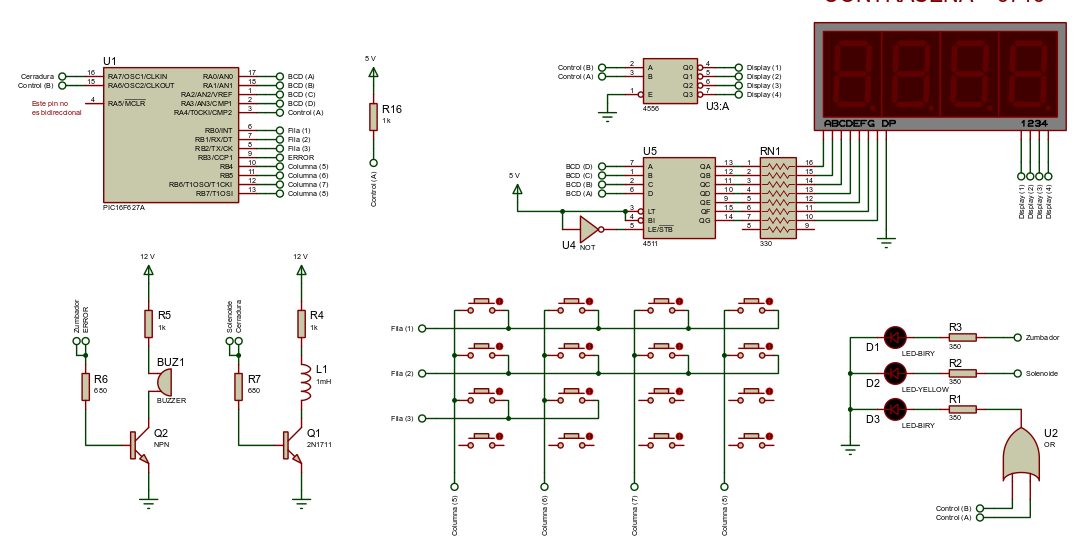
\includegraphics[width = \textwidth]{diagrama_esquematico.png}
	\caption{Diagrama esquematico hecho en Proteus}
\end{figure}

\section{Diagrama de flujo}
Este es el diagrama de flujo

\begin{figure}[H]
\centering
	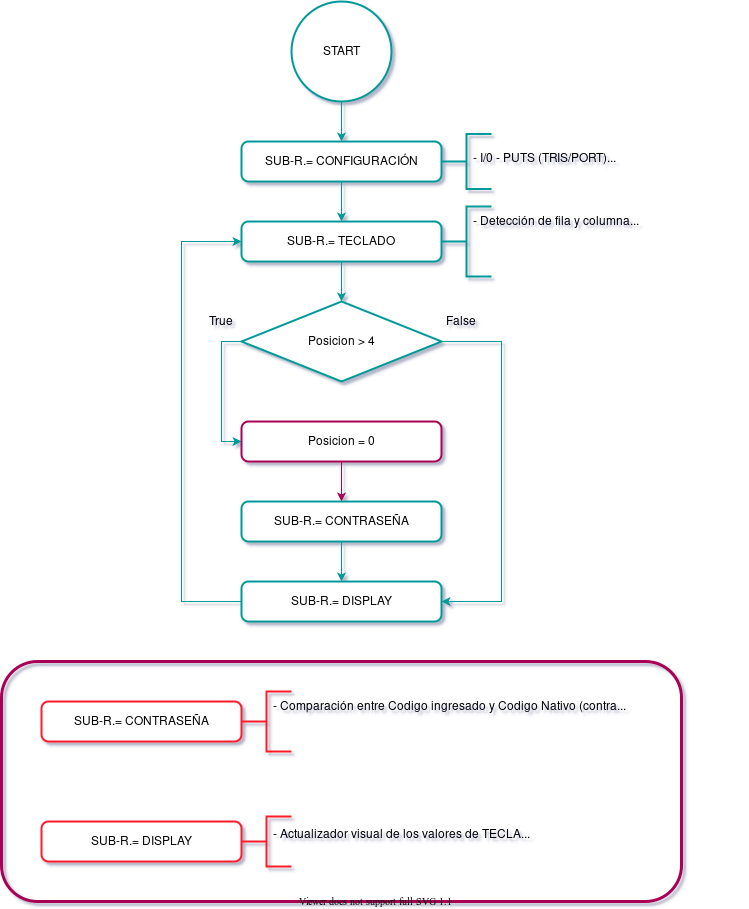
\includegraphics[width = 0.98\textwidth]{flujo_asm_general.png}
	\caption{Diagrama de flujo simplificado de assembler}
\end{figure}

\begin{figure}[H]
	\centering
	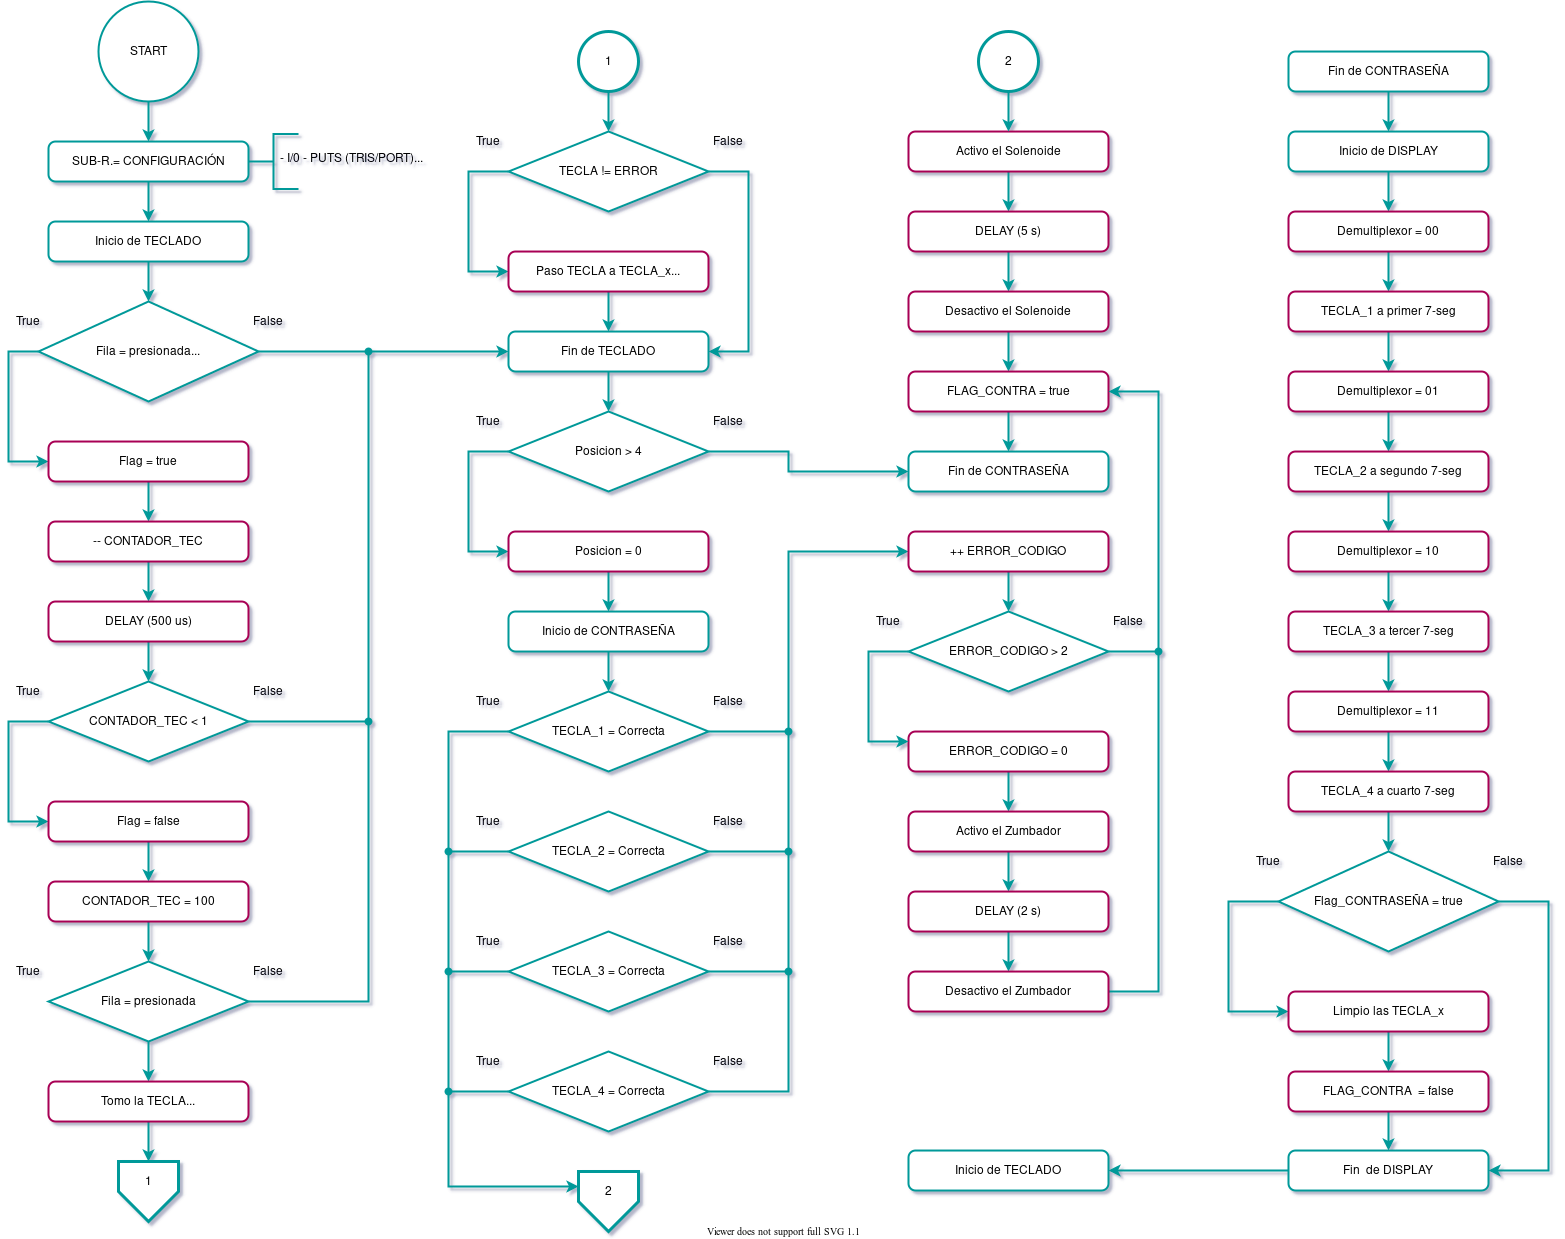
\includegraphics[width = \textwidth]{flujo_asm_completo.png}
	\caption{Flujo completo de assembler}
\end{figure}

\begin{figure}[H]
	\centering
	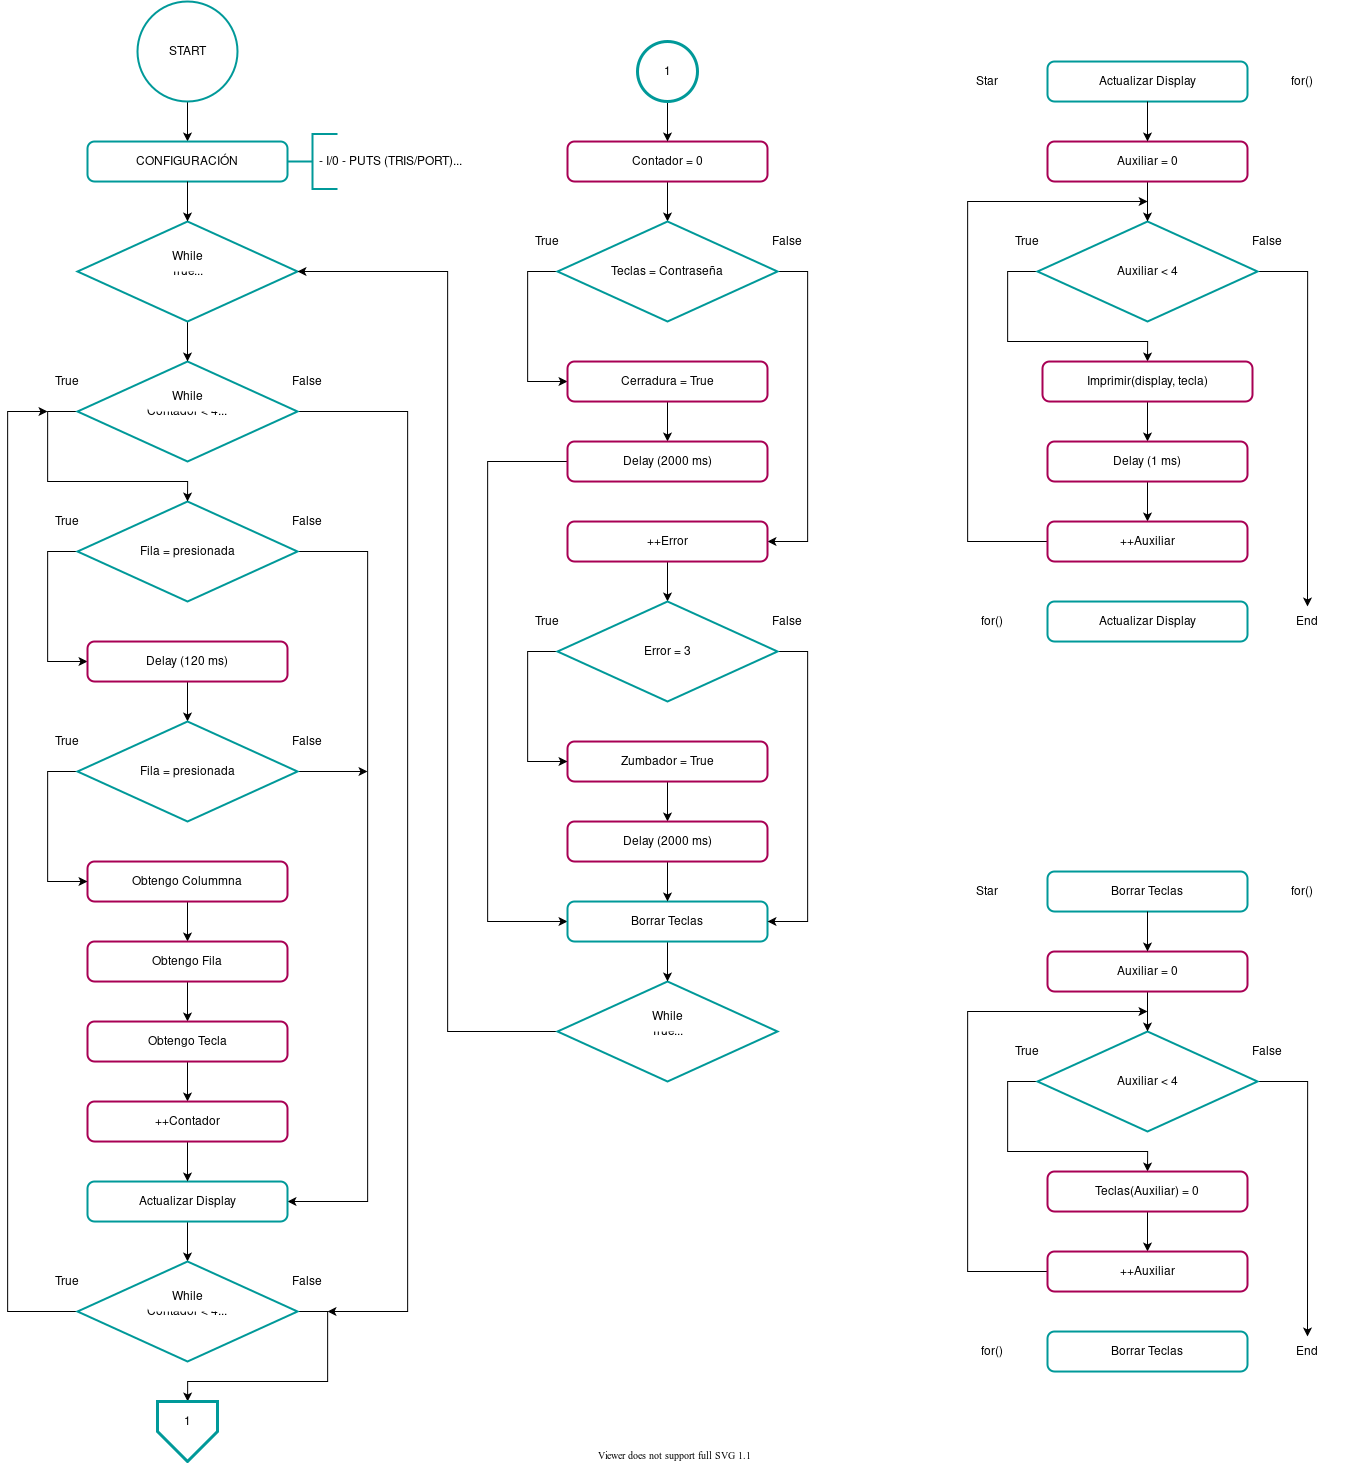
\includegraphics[width = \textwidth]{flujo_c.png}
	\caption{Flujo de C}
\end{figure}

\section{Código en assembler}

\inputminted
[frame= lines, linenos, breaklines, tabsize = 3, fontsize=\footnotesize, 
label=Codigo principal, fontseries=inconsolata]
{nasm}{codigo_asm.asm}

\section{Código en C}

\inputminted 
[frame= lines, linenos, breaklines, tabsize = 3, fontsize=\footnotesize, 
label=Codigo principal, fontseries=inconsolata]
{c}{codigo_c.c}

\section{Bitacoras personales}
	Con respecto al código en C, se empezó diseñando las funciones que serían de utilidad
	a la hora de realizar el código principal.

	Las que primero se diseñaron fueron las funciones que se utilizan para imprimir en el
	display de 7 segmentos, la cual fue diseñada para tener versatilidad para poder
	imprimir cualquier numero en cualquier display. Lo único que le falta a esa función es
	poder alternar entre modo cátodo común y ánodo común.
	
	Luego se diseñó el código que detecta que tecla se pulsó, y en un momento se hizo
	una función de delay\_ms() personalizada, que permite pasar variables como argumentos.

	Hubo problemas con la función de imprimir en los displays, y sucedió que teníamos los
	pines del decodificador mal colocados, entonces no recibía correctamente la información.

	Se hicieron las funciones pensando que tenían que ser lo más facil de entender posible,
	con nombres descriptivos y claros.
	Una cosa que se tuvo en mente es usar la filosofía UNIX, que es hacer una
	instrucción que haga una sola cosa y que la haga bien.

	El codigo en assembler fue dividido en multiples instrucciones, fue creado en base a un
	código preliminar hecho en pseudo-código.

\section{Simulaciones en Proteus}

	\subsection{ Assembler}
	\begin{itemize}
		\item \url{https://www.loom.com/share/57d7351ca74c480face7ed5f56e2720c?sharedAppSource=personal_library}\\
		\item \url{https://www.loom.com/share/4943de01fee7459e9b8c88f70fd844cd?sharedAppSource=personal_library}
	\end{itemize}

	\subsection{C}
	\begin{itemize}
		\item \url{ https://www.loom.com/share/e2184dde78ff4f12a691476db8c95cd1}
	\end{itemize}


\end{document}
